\subsection{Non-Rehabilitation Exoskeletons}

While rehabilitation exoskeletons are the primary focus of this dissertation, it is essential to note the innovation of exoskeletons designed for strength augmentation and reducing metabolic costs. The application of these exoskeletons ranges from military applications to construction and factory work. These exoskeletons can enhance the user's upper and lower body. Additionally, both soft and rigid exoskeletons have been explored.

In \cite{walsh2006autonomous} Walsh \textit{et. al} presented an under-actuated lower-limb exoskeleton that was able to transmit 90\% of the loads to the ground. Additionally, in \cite{wehner2013lightweight} and \cite{asbeck2013biologically} a soft lower limb exoskeleton was presented and examined, which was able to reduce the metabolic cost during a gait cycle. \autoref{fig:walsh} shows an example of a soft lower limb exoskeleton. These suits use actuated Bowden cables connected to the joints to help pull the joints through the gait cycle. While soft suites have the benefit of being lightweight, they do not provide structural support.  



As discussed above, the \textbf{BLEEX} was designed for military application to increase the load a person was able to carry and reduce the metabolic costs. The research was primarily funded by DARPA\footnote{https://www.darpa.mil/}.  Unlike the suite presented by Walsh, this suite is a rigid system with large powered actuators. \autoref{fig:BLEEX} shows the BLEEX military lower limb exoskeleton.


The \textbf{HAL-5} exoskeleton has both upper and lower body systems. \autoref{fig:HAL5} show the HAL-5 exoskeleton. This system was initially designed as a lower-body assistive device with the upper body; it allows users to increase their load caring capability. This system uses electromyogram (EMG) signals to detect the user's intent and provide assistance \cite{casolo2008active}.


\begin{figure}
     \centering
     \begin{subfigure}{0.5\textwidth}
    \centering
    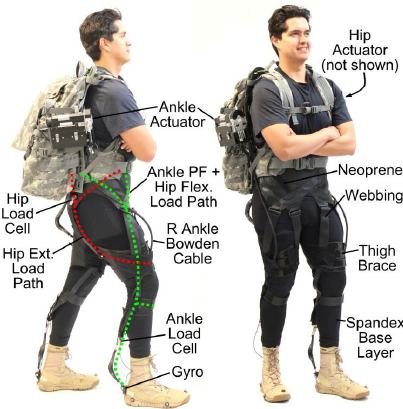
\includegraphics[width=.9\linewidth]{images/background/walsh.png}
    \caption[Walsh soft exoskeleton]{Walsh soft exoskeleton \cite{panizzolo2015evaluation}}
    \label{fig:walsh}
     \end{subfigure}
     \hfill
     \begin{subfigure}{0.3\textwidth}
        \centering
    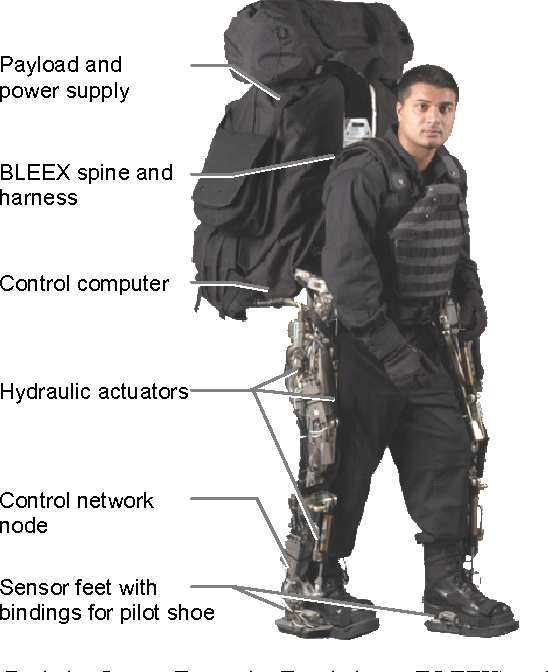
\includegraphics[width=.9\linewidth]{images/background/BLEEX2.png}
    \caption[BLEEX]{BLEEX powered exoskeleton for military applications \cite{kazerooni2006hybrid}}
    \label{fig:BLEEX}
     \end{subfigure}
     \begin{subfigure}{\textwidth}
           \centering
            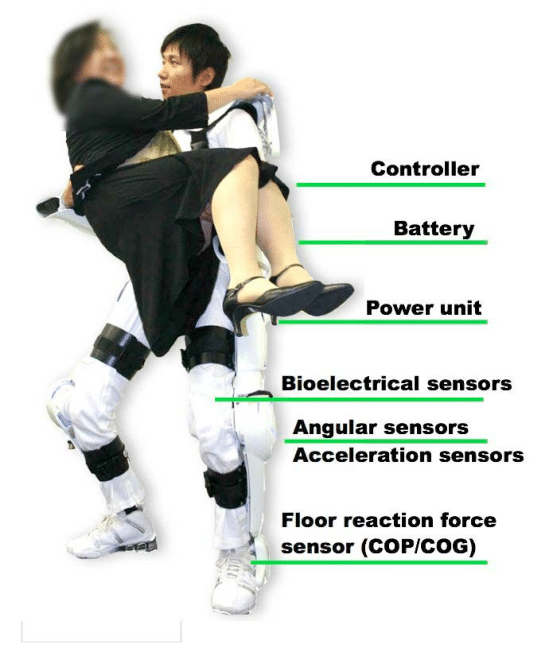
\includegraphics[width=.45\linewidth]{images/background/HAL-5.png}
        \caption[HAL-5]{HAL-5 exoskeleton \cite{sankai2010hal}}
    \label{fig:HAL5}
     \end{subfigure}
        \caption{Enactment Exoskeletons}
        \label{fig:enhanceExos}
\end{figure}

These exoskeletons have similar features as rehabilitation exoskeletons. They both need to be able to detect the user intent and provide assistive torques. However, it should be noted that soft exoskeletons do not provide structural support, which may be necessary if the person cannot support themselves. Additionally, detecting EMG signals maybe be plausible for people with SCI who, due to their injury.